\chapter{听觉处理的中枢神经系统}
听觉对于定位和识别声音至关重要; 对于人类来说,它特别重要,因为它在理解和产生语言方面发挥着重要作用。 听觉系统有几个值得注意的特征。 它的皮层下通路比其他感觉系统的通路更长。 与视觉系统不同,声音可以从四面八方进入听觉系统,白天和黑夜,无论我们睡着还是醒着。 听觉系统不仅处理从体外发出的声音(环境声音、他人发出的声音),还处理自己产生的声音(发声和咀嚼声音)。 声音刺激在空间中的位置不是由感觉传入神经元的空间排列来传达的,而是由听觉系统根据物理线索的表示来计算的。

\section{声音向有听觉的动物传达多种类型的信息}
听觉有助于提醒动物注意看不见的危险或机会的存在,而且在许多物种中,听觉还可以作为一种交流方式。 必须从每只耳朵的声音物理特性表示中提取有关声音从何处产生及其含义的信息。 要了解动物如何处理声音,首先要考虑哪些线索可用。

大多数脊椎动物利用两只耳朵来定位水平面上的声音。 在该平面上不同位置的声源对两只耳朵的影响不同:声音到达较早,并且在靠近声源的耳朵处更强烈(图\ref{localizing})。 双耳时间和强度差异携带有关声音出现位置的信息。

% !htb
\begin{figure}[htbp]
	\centering
	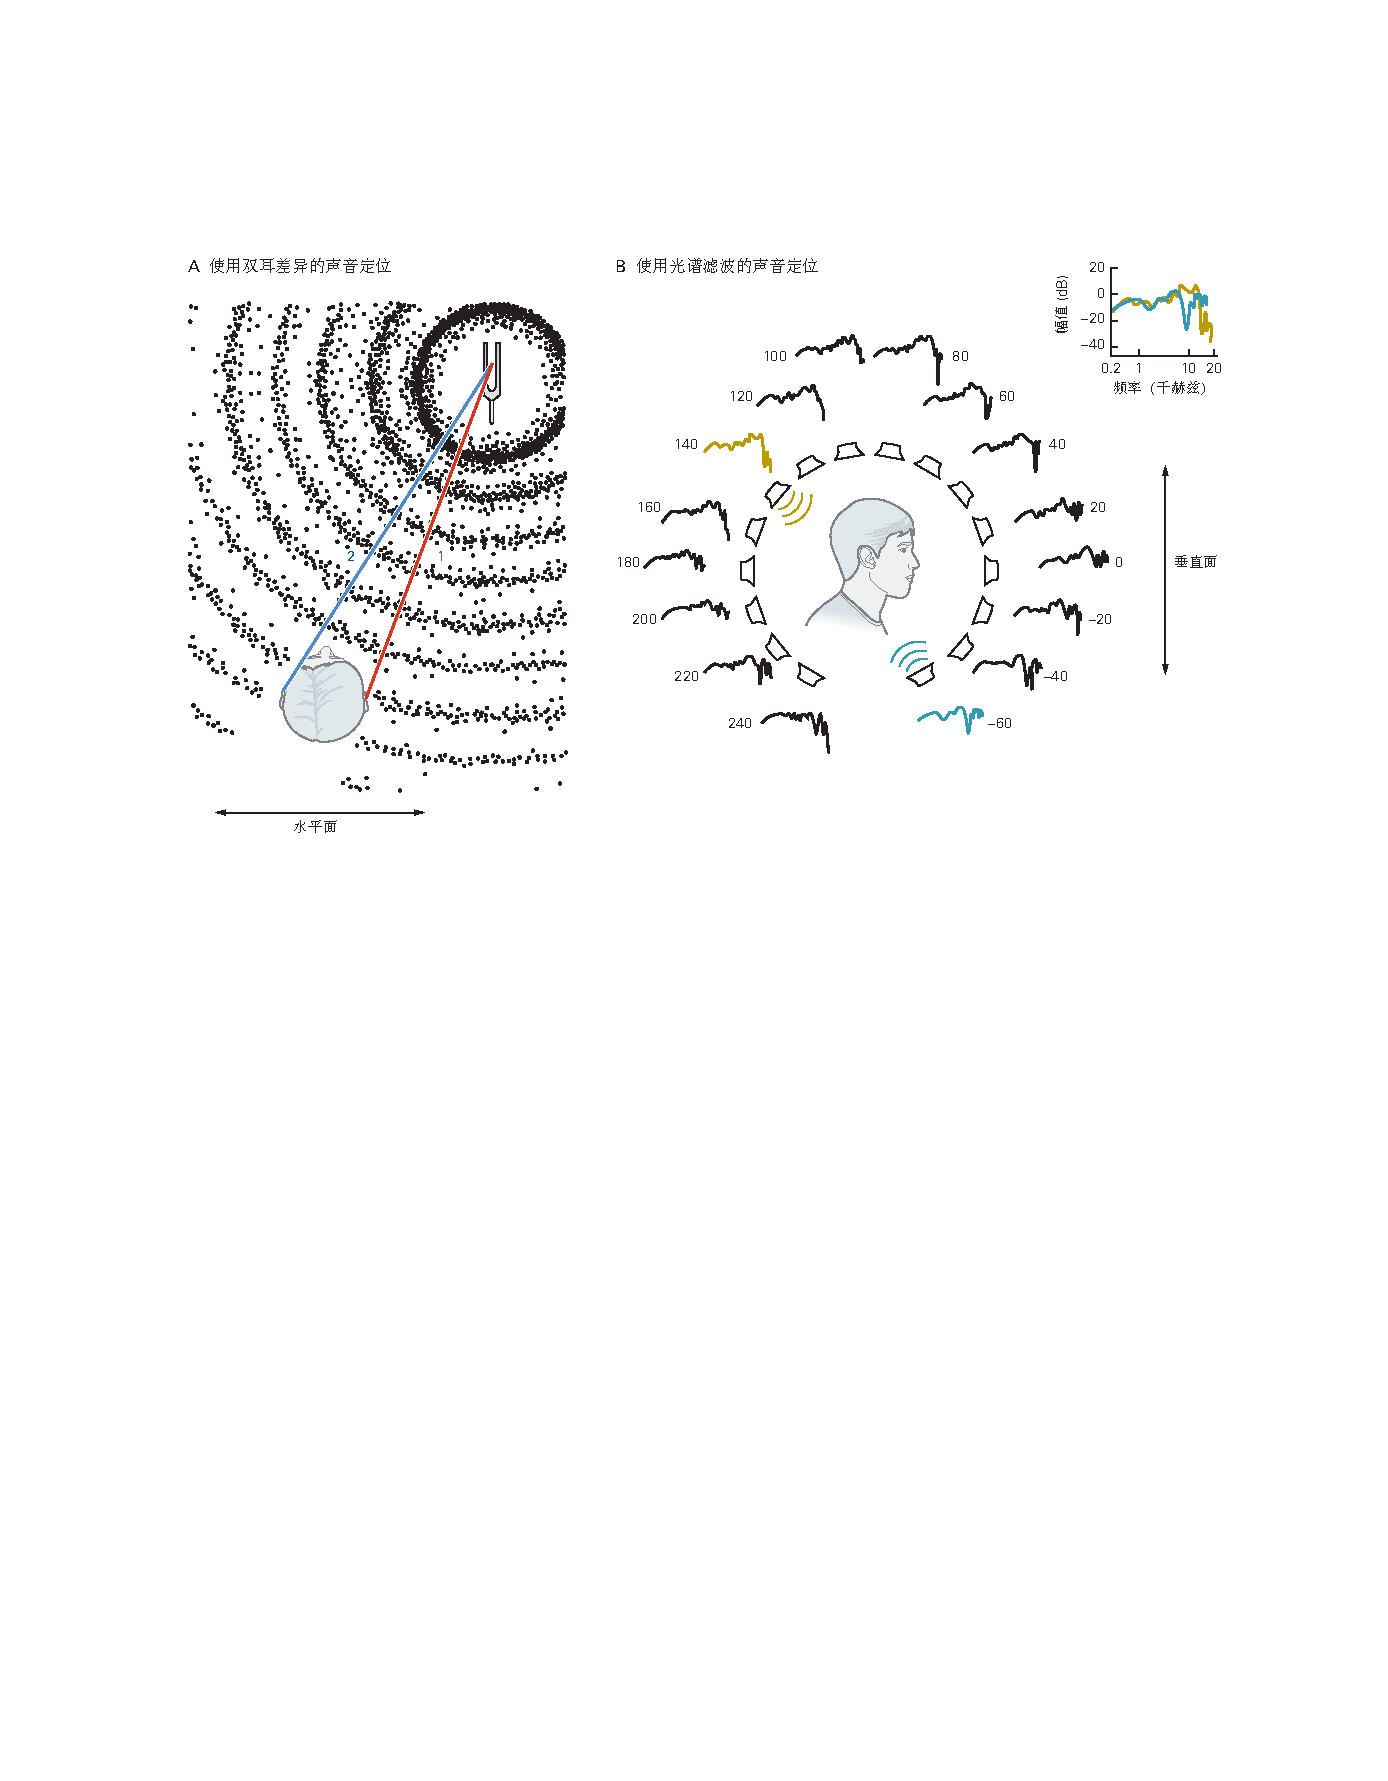
\includegraphics[width=1.0\linewidth]{chap28/fig_28_1}
	\caption*{在水平面上定位声源的提示。
		
	A. 双耳时间和强度差异是在水平面或方位角定位声源的线索。 在水平面上发出的声音到达两只耳朵的方式不同:声音到达的时间较早,并且越靠近声源的耳朵声音越大。 直接从前方或后方发出的声音到达左右耳的距离相同,因此同时到达双耳。 耳间时间和强度不随垂直平面中声源的移动而变化,因此不可能在垂直平面中定位纯正弦音调。 在人类中,最大的耳间时间差约为 600 微秒。 波长短的高频声音被头部偏转,在远处产生声影。 (经许可改编自 Geisler 1998。)

	B. 哺乳动物可以在频谱过滤的基础上在垂直和水平平面上定位宽带声音。 当通过扬声器呈现在人类听觉范围内的所有频率上都具有相同能量的噪声(白噪声)时,耳朵、头部和肩部会抵消某些频率的能量并增强其他频率的能量。 从扬声器发出的白噪声具有平坦的功率谱,但当噪声到达耳道底部时,其频谱不再平坦。

	在图中,耳膜处每个频率的声能相对于白噪声的声能由每个扬声器旁边的轨迹显示; 这些轨迹绘制了以分贝为单位的相对声音幅度与频谱频率(与头部相关的传递函数)的关系。 右上角的小图比较了两种与头部相关的传递函数:一种是针对听者前方出现的低噪声(蓝色),另一种是针对来自听者脑后的噪声(棕色)。 与头部相关的传递函数在大于 8 kHz 的频率处具有深陷波,其频率因声音的产生位置而异。 高频和窄带声音缺乏能量的声音很难在垂直平面上定位。 由于光谱过滤在水平面上也会发生变化,因此它为一只耳朵失去听力的动物提供了唯一的位置提示。

	您可以通过一个简单的实验来测试这些光谱线索的显着性。 闭上你的眼睛,当朋友在不同的高度直接在你面前叮当作响。 比较您在正常条件下定位声音的能力,以及当您通过用手指从后面推动双耳来扭曲双耳形状时的能力。 (数据来自 D. Kistler 和 F. Wightman。)}
	\label{localizing}
\end{figure}

头部的大小决定了耳间时间延迟与声源位置的关系; 神经元回路决定带时间延迟解析的精度。 由于气压波在空气中的传播速度约为 340 m/s,因此人类的最大耳间延迟约为 600 μs; 在小型鸟类中,最大延迟仅为 35 微秒。 人类可以将正前方声源的位置分辨到大约 1 度以内,对应于 10 微秒的耳间时间差。 编码相对较低频率的神经元特别能很好地传达双耳时间差异。 这些神经元可以在声音的每个周期中的相同位置发射,并以这种方式将耳间时间差编码为耳间相位差。 高频声音会在两只耳朵之间产生声影或强度差异。 对于许多头部较小的哺乳动物来说,高频声音是在水平面上定位声音的主要线索。

哺乳动物可以使用频谱滤波在垂直平面和单耳中定位声音。 高频声音的波长接近或小于头部、肩部和外耳的尺寸,与身体的这些部位相互作用产生相长和相消的干扰,引入宽谱峰和深而窄的谱槽,其频率 随声音的位置而变化(图 28-1B)。 来自不同来源的高频声音被不同地过滤,因为在哺乳动物中,外耳的形状从后到前以及从上到下不同。 动物学会使用这些光谱线索来定位声源。 如果通过实验改变耳朵的形状,即使是成年人也可以学会使用新的光谱线索模式。 如果动物的一只耳朵失去听力,它们就会失去耳间时间和强度线索,并且必须完全依赖光谱线索来定位声音。

我们如何理解我们听到的复杂多变的声音? 大多数自然声音都包含广泛频率范围内的能量,并随时间迅速变化。 用于识别声音的信息因动物种类而异,并且取决于聆听条件和经验。 例如,人类的语言可以在噪音中、通过扭曲声音的电子设备甚至通过人工耳蜗来理解。 其稳健性的一个原因是语音包含冗余线索:发声器官产生的声音中有多个参数是共变的。 与此同时,这使得理解动物如何识别模式成为一项复杂的任务。 目前尚不清楚动物在不同条件下会使用哪些线索。

音乐是人类快乐的源泉。 乐器和人声产生的声音在对应于其感知音高的基频以及该频率的倍数处具有能量,赋予声音一种质量,例如,当他们使用时,我们可以区分长笛和小提琴 音高是一样的。 音调主要在低频范围内,听觉神经纤维在这个范围内与声音同相发射。 在音乐中,声音同时组合产生和弦,并相继产生旋律。 悦耳、悦耳的和弦会在耳蜗神经纤维中引起规律、周期性的放电。 在不和谐的声音中,声音本身和听觉神经纤维的放电都不太规律; 分量频率非常接近,以至于它们相互干扰而不是周期性地相互增强。


\section{中央通路中声音的神经表征始于耳蜗核}
处理声学信息的神经通路从耳朵延伸到脑干,通过中脑和丘脑,到达大脑皮层(图 28-2)。 声学信息从耳蜗神经节中的细胞(见图 26-17)传送到脑干中的耳蜗核。 这些信息由几种不同类型的神经元接收,其中大多数神经元按音调排列。

\begin{figure}[htbp]
	\centering
	\includegraphics[width=1.0\linewidth]{chap28/fig_28_2}
	\caption*{中枢听觉通路从脑干通过中脑和丘脑延伸到听觉皮层。 耳蜗神经(颅神经 VIII)中的纤维终止于脑干的耳蜗核。 这些细胞核的神经元通过几条平行通路投射到下丘。 它们的轴突通过梯形体、中间听纹或背侧听纹退出。 一些细胞直接终止于下丘。 其他接触上橄榄复合体和外侧丘系细胞核中的细胞,后者又投射到下丘。 下丘的神经元投射到上丘和丘脑的内侧膝状体核。 丘脑神经元投射到听觉皮层。 耳蜗核和外侧丘系的腹侧核是唯一接收单耳输入的中枢听觉神经元。}
	\label{auditory_pathways}
\end{figure}

不同类型神经元的轴突采用不同的路径到达脑干和中脑,并在不同的目标处终止。 从耳蜗核到对侧下丘的一些通路是直接的; 其他涉及脑干听觉核中的一个或两个突触阶段。 从双侧下丘,声音信息以两种方式流动:到同侧上丘,在那里它参与调整头部和眼睛对声音的反应,以及到同侧丘脑,传递到大脑皮层的听觉区域。 从外围到更高脑区的传入听觉通路包括许多级别的传出反馈。

\subsection{耳蜗神经以平行途径将声学信息传递到音调组织的耳蜗核}
来自耳蜗神经节细胞的传入神经纤维被束缚在耳蜗或前庭耳蜗神经(脑神经 VIII)的听觉成分中,并完全终止于耳蜗核。 哺乳动物的耳蜗神经包含两组纤维:大量 (95\%) 的有髓纤维接收来自内毛细胞的输入,以及少量 (5\%) 的无髓纤维接收来自外毛细胞的输入。

与无髓纤维相比,更大、更多的有髓纤维更容易被理解。 每种类型都检测狭窄频率范围内的能量; 因此,耳蜗神经纤维的音调阵列携带着关于声音频率内容如何随时间变化的详细信息。 无髓神经纤维既终止于耳蜗腹侧核的大神经元,也终止于耳蜗腹侧核周围的小颗粒细胞。 因为很难从这些细小的纤维中记录下来,所以它们传递给大脑的信息还没有被很好地理解。 无髓神经纤维整合来自耳蜗相对广泛区域的信息,但对声音没有反应。 有人提出,这些纤维对耳蜗损伤有反应,并会导致听觉过敏——接触会损伤耳蜗的响亮声音后会感到疼痛。

耳蜗核的两个特征很重要。 首先,这些原子核按同位素组织。 携带来自检测低频的耳蜗顶端信息的纤维在腹侧和背侧耳蜗核的腹侧终止; 那些从检测高频的耳蜗基端携带信息的那些,在背侧终止(图 28-3)。 其次,每个耳蜗神经纤维支配耳蜗核内的几个不同区域,将具有不同投射模式的各种类型的神经元联系到更高的听觉中枢。 因此,听觉通路包括至少四个平行的上升通路,它们同时从耳蜗神经纤维携带的信号中提取不同的声学信息。 并联电路是脊椎动物感觉系统的一般特征。



\subsection{耳蜗腹核提取有关声音的时间和频谱信息}
无层腹侧耳蜗核的主要细胞可锐化时间和光谱信息,并将其传送到听觉通路的更高中心。 三种类型的神经元混合在一起,并通过脑干形成不同的通路(图 28-4)。

浓密细胞双侧投射到上橄榄复合体。 这条路有两部分。 一个穿过内侧上橄榄并比较声音到达两只耳朵的时间; 另一个穿过梯形体的内侧核和外侧上橄榄并比较耳间强度。 大的球形浓密细胞感知低频并双侧投射到内侧上橄榄,形成检测耳间时间延迟并有助于水平面低频声音定位的电路。 小球形浓密细胞和球状浓密细胞感知更高的频率。 小球形浓密细胞刺激同侧外侧上橄榄。 球状浓密细胞通过花萼末梢刺激梯形体对侧内侧核中的神经元,进而抑制外侧上橄榄的主要细胞。 外侧上橄榄中的神经元整合了同侧兴奋和对侧抑制,以测量耳间强度并定位水平面中的高频声音源(见图 28-6)。

星状细胞广泛终止。 它们兴奋同侧耳蜗背核的神经元,梯形体腹核中的内侧橄榄蜗传出神经元,同侧外侧上橄榄附近的橄榄周核,以及外侧丘系,下丘的对侧腹核, 和丘脑。 星状细胞的同位素阵列对声音的频谱进行编码。

章鱼细胞激发对侧橄榄旁核中的靶标,并终止于外侧丘系腹侧核神经元上的大兴奋性肾盏末梢,这反过来又对下丘提供了及时的甘氨酸能抑制。 章鱼细胞检测声音的开始,使动物能够检测到短暂的间隙。 它们标记来自一个来源的光谱成分,这些成分必须一起开始。

这些通路通过腹侧耳蜗核执行的综合任务的差异反映在细胞形态上。 它们的树突形状反映了它们从耳蜗神经纤维收集信息的方式。 高度调谐的浓密和星状细胞的树突从相对较少的耳蜗神经纤维接收输入,而相比之下,广泛调谐的章鱼细胞的树突垂直于耳蜗神经纤维的路径,准备接收来自许多耳蜗神经纤维的输入 . 浓密细胞的许多输入来自包裹浓密细胞体的异常大的终端,满足它们对大突触电流的需要。 章鱼细胞对大突触电流的需求是通过对来自大量小终端的输入求和来满足的。

神经元的生物物理学特性决定了突触电流如何转化为电压变化,以及突触输入被整合的时间长短。 腹侧耳蜗核中的章鱼和浓密细胞能够以异常快速和精确定时的突触电位做出反应。 这些神经元具有显着的低电压激活 K+ 电导,可提供低输入电阻和快速响应并防止重复放电(图 28–4C)。 在这些渗漏细胞中触发动作电位所需的大突触电流通过许多突触处的快速门控、高电导、AMPA 型(α-氨基-3-羟基-5-甲基异恶唑-4-丙酸盐)谷氨酸受体传递 发布网站。 相比之下,即使相对较小的去极化电流也会产生较大的持续电压变化的星状细胞会响应突触电流而产生较慢的兴奋性突触后电位 (EPSP),而 N-甲基-d-天冬氨酸 (NMDA) 型谷氨酸受体会增强这些响应。


\subsection{耳蜗背核将声学与体感信息相结合,利用频谱线索定位声音}

在脊椎动物中,只有哺乳动物具有背侧耳蜗核。 耳蜗背核接收来自投射到不同层的两个神经元系统的输入(图 28–4A、B)。 它的主要细胞梭形细胞整合了这两个输入系统,并将结果直接传送到对侧下丘。

最外层的分子层是平行纤维系统的末端,颗粒细胞的无髓鞘轴突散布在耳蜗核内和周围。 该系统将体感、前庭和听觉信息从大脑的广泛区域传输到分子层。

深层接收声音信息。 不仅耳蜗神经纤维而且腹侧耳蜗核的星状细胞也终止于深层。 声学输入按音调分布在与平行纤维成直角的等频层中。

梭形细胞是耳蜗背核的主要细胞,整合了两个输入系统。 分子层中的平行纤维通过分子层顶端树突上的刺激发梭形细胞。 平行纤维也终止于车轮细胞的树突棘,中间神经元与小脑浦肯野细胞非常相似,后者反过来抑制梭状细胞。 腹侧耳蜗核中的耳蜗神经纤维和星状细胞通过深层光滑基底树突上的突触激发梭状细胞和抑制性中间神经元。

最近的实验表明,耳蜗背核的回路可以区分不可预测和可预测的声音。 例如,动物自己的咀嚼或舔舐声音是可以预测的,并通过这些电路消除。 当动物移动头部、耳朵或肩膀时出现的光谱线索变化,改变了声音入射到耳朵的角度,这是不可预测的,尤其是当外部声源移动时。 关于头部和耳朵位置的体感和前庭信息,以及来自更高层次神经系统的关于动物自身运动的下行信息,通过分子层调制到达深层的声学信息。

\section{哺乳动物的上橄榄复合体包含用于检测耳间时间和强度差异的独立电路}
在许多脊椎动物中,包括哺乳动物和鸟类,上橄榄复合体中的神经元比较双侧耳蜗核中细胞的活动以定位声源。 单独的电路检测耳间时间和强度差异并投射到下丘。

\subsection{内侧上橄榄生成耳间时差图}
\subsection{外侧上橄榄检测耳间强度差异}
\subsection{上橄榄复合体向耳蜗提供反馈}
\subsection{下丘外侧丘系形状响应的腹侧核和背侧核抑制}

\section{传入听觉通路在下丘汇聚}
\subsection{来自下丘的声音位置信息在上丘中创建声音的空间图}

\section{下丘传输声音信息给大脑皮层}
\subsection{沿着上行通路刺激选择性逐渐增加}
\subsection{听觉皮层映射众多的声音方位}
\subsection{从下丘而来的第二声音定位通路涉及凝视控制的大脑皮层}
\subsection{大脑皮层中的听觉回路被分离成分开的处理流}
\subsection{大脑皮层在皮下听区调制感觉加工}

\section{大脑皮层形成复杂的声音表示}
\subsection{听觉皮层使用时间和速率编码来表征时变声音}
\subsection{灵长类有专门的皮层神经元编码音高和泛音}
\subsection{食虫蝙蝠有皮层区域专门负责行为相关的声音特征}
\subsection{听觉皮层涉及处理说话时的声音反馈}

\section{要点}
\subsection{选读}
\subsection{参考文献}
